\section{方案论证}
\subsection{结构概述}
弹簧管压力表是一种用来测量气体压力的仪表。
\newline
压力表的组成:
\begin{itemize}
    \item 灵敏部分(弹簧管)
    \item 传动放大部分(曲柄滑块、齿轮机构)
    \item 示数部分(指针、刻度盘)
    \item 辅助部分(游丝)
\end{itemize}
\subsubsection{灵敏元件}
将不便测量的物理量转换成易于直接比较的物理量,本设计将弹簧管作为灵敏元件,将不易于比较的压力转换为易于测量的位移.
\subsubsection{传动放大机构}
本设计由曲柄滑块机构和齿轮传动机构组成.目的在于传递或放大位移,改变位移性质和得到等分刻度,并且应具有一定的补偿特性,同时仪表有较好的线性特性.
\subsubsection{示数装置}
其作用是在接受传动放大机构的位移后,指示出待测量的数值.本设计采用指针指示标尺刻度.
\subsubsection{辅助装置}
其作用是保持仪表传动系统单向接触,消除空回,消除齿轮、铰销产生的回差。
\subsection{原理分析}
作为灵敏元件的弹簧管可以把气体压力转变为管末端的位移,通过曲柄滑块机构将此位移转变为曲柄的转角,然后通过齿轮机构将曲柄转角放大,带动指针偏转,从而指示压力的大小。将转角放大便于测量,可以提高测量精度。压力表工作原理和框图如\autoref{FIGURE2.1}和\autoref{FIGURE2.2}所示。
\begin{figure}[!htbp]
    \centering
    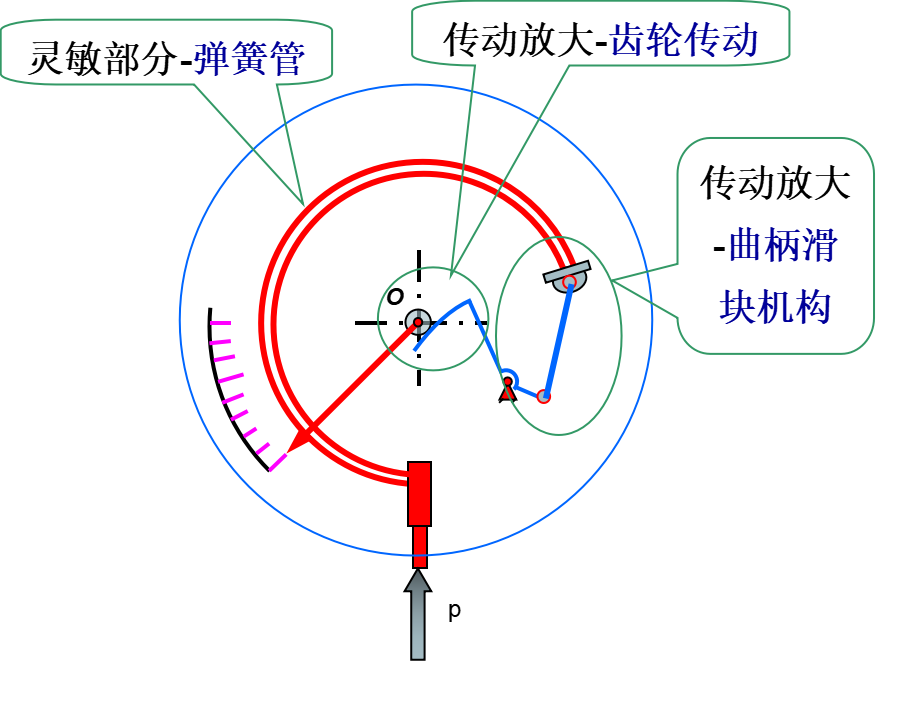
\includegraphics[width =0.5\textwidth]{figures/2.1.png}
    \caption{压力表工作原理}
    \label{FIGURE2.1}
\end{figure}
\begin{figure}[!htbp]
    \centering
    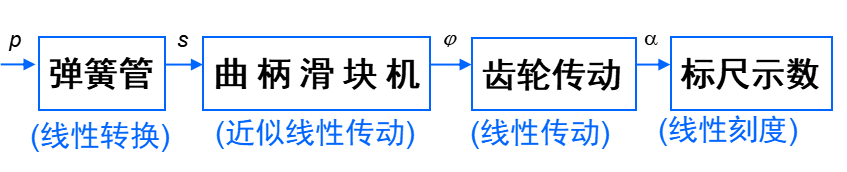
\includegraphics[width =\textwidth]{figures/2.2.png}
    \caption{压力表工作原理框图}
    \label{FIGURE2.2}
\end{figure}
\newpage
弹簧管的压力-位移是线性关系,但弹簧管本身的工艺问题(如材料、加工等)会造成一些线性误差,弹簧管形状的不直、不均匀也会导致非线性误差。曲柄滑块机构可以补偿弹簧管的线性及非线性误差。从$0{\sim}0.4Mpa$调整满足满刻度精度为线性误差调整,中间部分不均匀调整为非线性误差调整。

% \subsection{弹簧管}
% 将不便测量的物理量转换成易于直接比较的物理量,本设计将弹簧管作为灵敏元件,将不易于比较的压力转换为易于测量的位移.
% \subsection{曲柄滑块机构}
% 将弹簧管的非线性位移通过曲柄滑块机构转化成齿轮的线性转动。
% \subsection{齿轮传动}
% 通过设计两个齿轮的中心距,选定模数、小齿轮齿数,大齿轮的扇形角,大小齿轮的分度圆直径,尺顶圆直径,齿根圆直径来达到恒定传动比,将曲柄滑块的线性角度传动传动到指针转动的角度。
% \subsection{游丝}
% 游丝属于平面涡卷弹簧,它是由金属带材在一个平面内绕成的螺旋线形状的一种惯性元件,游丝工作时其外端固定在机壳上,内端固定在转轴上,随转轴一起旋转,游丝承受转矩而盘紧,放松时产生反作用力而工作,游丝在工作中时各圈之间是不接触的。游丝的功能是保持仪表传动系统单向接触,消除齿轮。铰销消除产生的回差。
% \subsection{标尺指针}
